\documentclass[11pt]{article}
\bibliographystyle{plain}
\usepackage{geometry} % see geometry.pdf on how to lay out the page. There's lots.
\usepackage{amsmath,amssymb} 
\usepackage{epsfig,epsf,subfigure,array}
\geometry{a4paper} 

%\setlength{\parindent}{0pt}
%\setlength{\parskip}{1ex plus 0.5ex minus 0.2ex}

\newcommand{\dif}{\, \mathrm{d}}
\newcommand{\diff}[2]{\frac{\mathrm{d}#1}{\mathrm{d}#2}}
\newcommand{\partdiff}[2]{\frac{\partial #1}{\partial #2}}

\begin{document}
 
\LARGE
\begin{center}
TMA4280: Introduction to Supercomputing
\end{center}
\vspace{1in}

\begin{center}
{\bf The Poisson problem in $\mathbb{R}^2$: \\
diagonalization methods}
\end{center}

\Large
\vspace{0.5in}
\begin{center}
Spring 2014
\end{center}

\vspace{0.5in}

\begin{center}
\copyright Einar M. R{\o}nquist \\
Department of Mathematical Sciences\\
NTNU, N-7491 Trondheim, Norway\\
All rights reserved \\
Revised by Arne Morten Kvarving, 2014
\end{center}

\large

\newpage

\section{Direct method based on diagonalization}
Let us now consider a different way of solving the finite difference equations
we derived in the context of discretizing the Poisson problem. 
The method is based on {\em diagonalization}, and we first explain the approach 
in the context of the one-dimensional Poisson problem:

\begin{align*}
  -u_{xx} &= f \quad \text{in } \Omega = (0,1), \\
  u(0) = u(1) &= 0.
\end{align*}
Assume that we use a uniform finite difference {\em grid} given by:
\begin{equation*}
  x_i = x_0 + ih, \quad i=0,1,\ldots,n.
\end{equation*}

The corresponding system of algebraic equations can be written as:

\begin{align*}
  \frac{1}{h^2}
  \begin{bmatrix}
    2 & -1 & & & \\
    -1 & 2 & -1 & & \\
    & -1 & 2 & -1 & \\
    & & & \ddots & -1 \\
    & & & -1 & 2
  \end{bmatrix}
  \begin{bmatrix}
    u_1 \\
    u_2 \\
    \vdots \\
    \vdots \\
    u_{n-1}
  \end{bmatrix}
  =
  \begin{bmatrix}
    f_1 \\
    f_2 \\
    \vdots \\
    \vdots \\
    f_{n-1} 
  \end{bmatrix}, \\ 
\end{align*}
where $u_i$ is an approximation to $u(x_i) = u(ih), \quad i=1,\ldots,n-1$, 
$f_i=f(x_i)$, and $u_0 = u_n=0$ due to the specified boundary conditions. 
Let us write this system as

\begin{align*}
  \frac{1}{h^2}\, \underline{T} \, \underline{u} &= \underline{f} 
\end{align*}
where 
\begin{align*}
  \underline{T} = 
  \begin{bmatrix}
    2 & -1 & & & \\
    -1 & 2 & -1 & & \\
    & -1 & 2 & -1 & \\
    & & & \ddots & -1 \\
    & & & -1 & 2
  \end{bmatrix} , \qquad 
  \underline{u} =
  \begin{bmatrix}
    u_1 \\
    \vdots \\
    \vdots \\
    \vdots \\
    u_{n-1}
  \end{bmatrix} , \qquad
  \underline{f} =
  \begin{bmatrix}
    f_1 \\
    \vdots \\
    \vdots \\
    \vdots \\
    f_{n-1}
  \end{bmatrix} ,
\end{align*}
and $h$ is the grid size or mesh size. Since $\underline{T}$ is symmetric positive definite, it can be {\em diagonalized}.

\subsection{Diagonalization of $\underline{T}$}

Diagonalization of $\underline{T}$ means that we wish to find the 
eigenvalues $\lambda_j$ and the eigenvectors $\underline{q}_j$ 
of $\underline{T}$, 
\begin{align*}
  \underline{T}\, \underline{q}_j &= \lambda_j \,\underline{q}_j, \quad j=1,\ldots,n-1 ,\\
  \intertext{where}
  \lambda_j &> 0 \qquad \text{(positive eigenvalues)}, \\
  \underline{q}_k^T \underline{q}_j &= \delta_{jk} \qquad \text{(orthonormal eigenvectors)}.
\end{align*}

We collect all the eigenvectors $\underline{q}_j$ into the (orthonormal) 
matrix $\underline{Q}$,

\begin{equation*}
  \underline{Q} = [\underline{q}_1, \underline{q}_2,\ldots,\underline{q}_{n-1}].
\end{equation*}
Then

\begin{align*}
  \underline{T} \, \underline{Q} &= \underline{Q} \, \underline{\Lambda}, \\
  \intertext{where}
  \underline{\Lambda} &= \text{diag}(\lambda_1, \ldots, \lambda_{n-1}) = 
  \begin{bmatrix}
    \lambda_1 & & & \\
     & \ddots & & \\
    & & \ddots & \\
    & & & \lambda_{n-1}
  \end{bmatrix}. 
\end{align*}
Since
\begin{align*}
  \underline{Q}^T \underline{Q} = \underline{I} = 
  \begin{bmatrix}
    1 & & & \\
     & \ddots & & \\
    & & \ddots & \\
    & & & 1
  \end{bmatrix} \qquad
  \Rightarrow \quad \underline{Q}^T = \underline{Q}^{-1} ,
\end{align*}
and
\begin{align}
  \underline{T} &= \underline{Q} \,\underline{\Lambda} \,\underline{Q}^T 
  \label{eq:T_diag}
\end{align}
or 
\begin{align*}
  \underline{Q}^T\, \underline{T} \, \underline{Q} &= \underline{\Lambda} \qquad \text{(diagonal)}.
\end{align*}

\newpage

Following this approach the finite difference approximation can be computed as follows:

\begin{alignat*}{2}
  \underline{g} &\equiv  h^2 \underline{f} \quad &  \qquad \qquad \underline{g} &: \mathcal{O}(n) \text{ operations} \\ \\
  \underline{T} \, \underline{u} &= \underline{g} \\
  \underline{Q} \, \underline{\Lambda} \, \underline{Q}^T \underline{u} &= \underline{g} \\
  \underline{\Lambda}\, \underset{\widetilde{\underline{u}}}{\underbrace{\underline{Q}^T\, \underline{u}}} &= \underset{\widetilde{\underline{g}}}{\underbrace{\underline{Q}^T \underline{g}}} & \widetilde{\underline{g}} &: \mathcal{O}(n^2) \text{ operations} \\ \\
  \underline{\Lambda} \widetilde{\underline{u}} &= \widetilde{\underline{g}} \\
  \widetilde{\underline{u}} &= \underline{\Lambda}^{-1} \widetilde{\underline{g}} & \widetilde{\underline{u}} &: \mathcal{O}(n) \text{ operations} \\
  \underline{Q}^T \underline{u} &= \widetilde{\underline{u}} \\
   \underline{u} &= \underline{Q} \, \widetilde{\underline{u}} & \underline{u} &: \mathcal{O}(n^2) \text{ operations} \\
\end{alignat*}
Note that the transformations
\begin{equation*}
  \widetilde{\underline{g}} = \underline{Q}^T \underline{g} \text{ and } \underline{u} = \underline{Q} \, \widetilde{\underline{u}}
\end{equation*}
are {\em matrix-vector products operations}.
In summary, we can compute $\underline{u}$ in
\begin{equation*}
  \mathcal{O}(n) + \mathcal{O}(n^2) + \mathcal{O}(n) + \mathcal{O}(n^2) \sim \mathcal{O}(n^2) \text{ floating-point operations}.
\end{equation*}
Hence, we can solve our finite difference system in $(n-1)$ unknowns in $\mathcal{O}(n^2)$ operations. This is {\em not} competitive with a direct solution algorithm based upon LU-factorization (Gaussian elimination) of a tridiagonal matrix, which can be done in $\mathcal{O}(n)$ operations (since the bandwidth is equal to one).\\

Let us also compare the memory requirement:
\begin{align*}
  &\mathcal{O}(n^2) \text{ for the diagonalization approach 
  (we need to store $\underline{Q}$)}; \\
  &\mathcal{O}(n) \text{ for a tridiagonal direct solver}.
\end{align*}
Again, the diagonalization approach is {\em not} competitive.

So, why bother?  The answer is that the diagonalization approach becomes 
more interesting in $\mathbb{R}^2$. In addition, we will later see how we 
can use the Fast Fourier Transform (FFT) to lower the computational complexity. 



\section{The Poisson problem in $\mathbb{R}^2$}

The two-dimensional Poisson problem on the unit square is given by

\begin{equation}
  \begin{split}
    -\nabla^2 u &= f \qquad \text{in } \Omega=(0,1) \times (0,1), \\
    u &= 0 \qquad \text{on } \partial \Omega, \\
  \end{split}
  \label{eq:Poisson2D}
\end{equation}

where $\nabla^2 u = \frac{\partial^2 u}{\partial x^2} + \frac{\partial^2 u}{\partial y^2}$.


\begin{figure}[h]
  \centering
  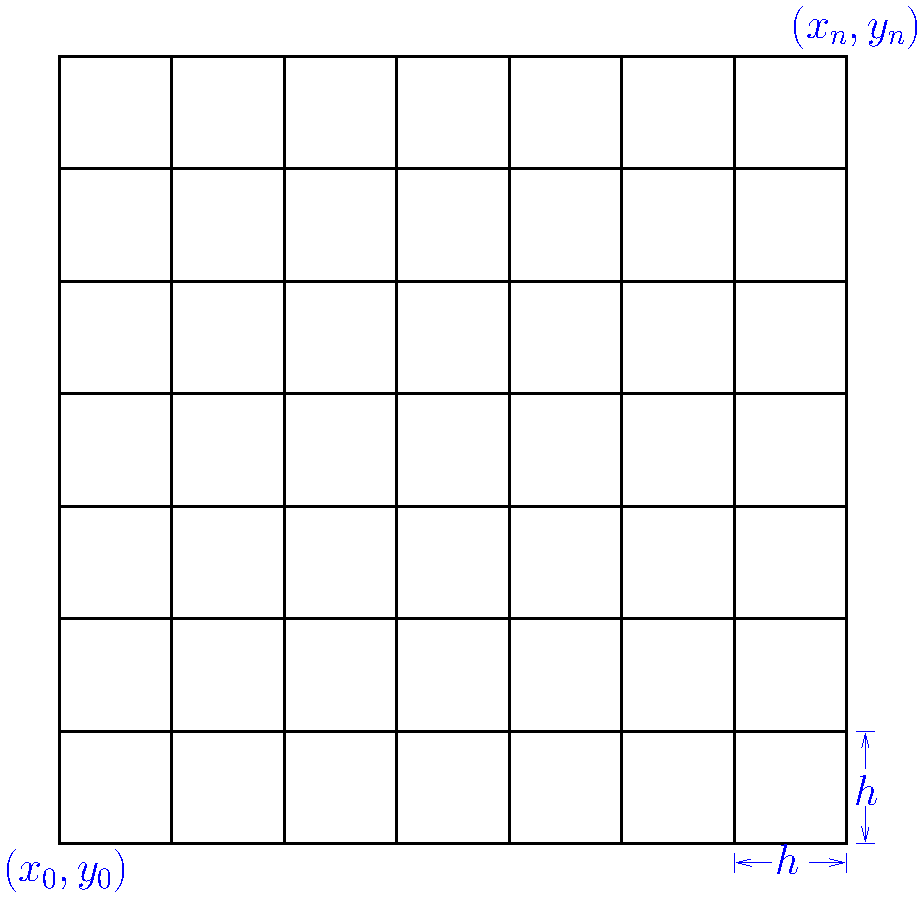
\includegraphics[width=8cm]{FiniteDifferenceGrid}
    \caption{A uniform finite difference grid.}
  \label{fig:FDM_grid_2D}
\end{figure}

Again, using the notation $u_{i,j} \simeq u(x_i,y_j) = u(i h, j h)$ and $f_{i,j}=f(x_i,y_j)$,
and discretizing \eqref{eq:Poisson2D} using the 5-point stencil (see Figure \ref{fig:FDM_grid_2D}), the discrete equations read:

\begin{equation}
  -\frac{(u_{i+1,j}-2u_{i,j}+u_{i-1,j})}{h^2} - \frac{(u_{i,j+1}-2u_{i,j}+u_{i,j-1})}{h^2} = f_{i,j} ,\qquad 1 \leq i,j \leq n-1.
  \label{eq:FDM_sys}
\end{equation}

\subsection{Diagonalization}
Let 

\begin{equation*}
  \underline{{U}} = 
  \begin{bmatrix}
    u_{1,1} & \ldots & \ldots & u_{1,n-1} \\
    \vdots & & & \vdots \\
    \vdots & & & \vdots \\
    u_{n-1,1} & \ldots & \ldots & u_{n-1,n-1}
  \end{bmatrix}
\end{equation*}
and

\begin{equation*}
  \underline{{T}} = 
  \begin{bmatrix}
    2 & -1 & & & 0 \\
    -1 & 2 & -1 & & \\
    & & \ddots & & \\
    & & -1 & 2 & -1 \\
    0 & & & -1 & 2
  \end{bmatrix}
\end{equation*}

Then,

\begin{alignat*}{2}
  (\underline{{T}} \, \underline{{U}})_{ij} &= 2u_{i,j} - u_{i+1,j}, &\qquad &i=1, \\
  (\underline{{T}} \, \underline{{U}})_{ij} &= -u_{i-1,j}+2u_{i,j} - u_{i+1,j}, &\qquad 2 \leq &i \leq n-2, \\
  (\underline{{T}} \, \underline{{U}})_{ij} &= -u_{i-1,j}+2u_{i,j}, &\qquad &i=n-1.
\end{alignat*}

and thus,

\begin{equation}
  \boxed{\frac{1}{h^2} (\underline{{T}} \, \underline{{U}})_{ij} \simeq -\biggl( \frac{\partial^2 u}{\partial x^2} \biggr)_{i,j}. }
\end{equation}

Similarly,

\begin{equation}
  \boxed{\frac{1}{h^2} (\underline{{U}} \, \underline{{T}})_{ij} \simeq -\biggl( \frac{\partial^2 u}{\partial y^2} \biggr)_{i,j}. }
\end{equation}
\vspace{.2in}

Our finite difference system (\ref{eq:FDM_sys}) can thus be expressed as

\begin{equation*}
  \frac{1}{h^2} ( \underline{{T}} \, \underline{{U}} + \underline{{U}} \, \underline{{T}})_{ij} = f_{i,j} \qquad \text{ for } \qquad
  \begin{matrix}
    1 \leq i \leq n-1, \\
    1 \leq j \leq n-1,
  \end{matrix}
\end{equation*}

or 

\begin{equation}
  \underline{{T}} \, \underline{{U}} + \underline{{U}} \, \underline{{T}} = \underline{{G}}
  \label{eq:Poisson2D_TUUT}
\end{equation}

where

\begin{equation*}
  \underline{{G}} = h^2
  \begin{bmatrix}
    f_{1,1} & \ldots & \ldots & f_{1,n-1} \\
    \vdots & & & \vdots \\
    \vdots & & & \vdots \\
    f_{n-1,1} & \ldots & \ldots & f_{n-1,n-1}
  \end{bmatrix} .
\end{equation*}

\newpage
Combining (\ref{eq:T_diag}) and (\ref{eq:Poisson2D_TUUT}) we get

\begin{equation}
  \underline{{Q}}\, \underline{{\Lambda}}\, \underline{{Q}}^T \underline{{U}} + \underline{{U}}\, \underline{{Q}}\, \underline{{\Lambda}} \,\underline{{Q}}^T = \underline{{G}}.
  \label{eq:Poisson2D_T_diag}
\end{equation}

Multiplying (\ref{eq:Poisson2D_T_diag}) from the right with $\underline{{Q}}$ and from the left with $\underline{{Q}}^T$, and using the fact that 
$\underline{Q}^T\underline{Q} = \underline{I}$, we get:

\begin{equation*}
  \underline{{\Lambda}} \,\underset{\equiv \underline{{\widetilde{U}}}}{\underbrace{\underline{{Q}}^T\, \underline{{U}}\, \underline{{Q}}}} + \underset{\equiv \underline{{\widetilde{U}}}}{\underbrace{\underline{{Q}}^T\, \underline{{U}}\, \underline{{Q}}}}
\underline{{\Lambda}} = \underset{\equiv \underline{{\widetilde{G}}}}{\underbrace{\underline{{Q}}^T\, \underline{G}\, \underline{{Q}}}}.
\end{equation*}

Hence, (\ref{eq:Poisson2D_TUUT}) may be solved in three steps:\\ \\


\underline{\textbf{Step 1)}}: Compute

\begin{equation*}
  \boxed{ \underline{{\widetilde{G}}} = \underline{{Q}}^T\, \underline{{G}}\, \underline{{Q}} } \quad - \quad  
  \begin{matrix}
    \text{matrix-matrix} \\
    \text{products}.
  \end{matrix} \\
\end{equation*}

\underline{\textbf{Step 2)}}: Solve

\begin{align*}
  \underline{{\Lambda}} \, \underline{{\widetilde{U}}} + \underline{{\widetilde{U}}} \, \underline{{\Lambda}} = \underline{{\widetilde{G}}} & \\
  \intertext{or}
  \lambda_i \,\widetilde{u}_{i,j} + \widetilde{u}_{i,j}\, \lambda_j = \widetilde{g}_{i,j},  \qquad &1 \leq i,j \leq n-1 \\
  (\lambda_i + \lambda_j)\, \widetilde{u}_{i,j} = \widetilde{g}_{i,j},  \qquad &1 \leq i,j \leq n-1 \\
  \boxed{ \widetilde{u}_{i,j} = \frac{\widetilde{g}_{i,j}}{\lambda_i + \lambda_j}} \qquad &1 \leq i,j \leq n-1. \\
\end{align*}

\underline{\textbf{Step 3)}}: Compute 

\begin{equation*}
  \boxed{ \underline{{U}} = \underline{{Q}}\, \underline{{\widetilde{U}}} \,\underline{{Q}}^T } \quad - \quad  
  \begin{matrix}
    \text{matrix-matrix} \\
    \text{products}.
  \end{matrix}
\end{equation*}

Here,

\begin{equation*}
  \underline{{U}}, \underline{{\widetilde{U}}}, \underline{{\widetilde{G}}}, \underline{{Q}}, \underline{{Q}}^T \in \mathbb{R}^{(n-1) \times (n-1)}.
\end{equation*}


\subsubsection{Computational cost}

The number of degrees-of-freedom (or unknowns), $N$, is
\begin{align*}
N = (n-1)^2 \sim \mathcal{O}(n^2) \quad (n \gg 1).\\
\end{align*}

\underline{\textbf{Step 1)}}

\begin{equation*}
  \underline{{\widetilde{G}}} = \overset{\mathcal{O}(n^3)}{\overbrace{\underline{{Q}}^T \underset{\mathcal{O}(n^3)}{\underbrace{\underline{{G}}\, \underline{{Q}}}}}} \qquad \longrightarrow \qquad \mathcal{O}(n^3) \text{ operations}.
\end{equation*}

\underline{\textbf{Step 2)}}

\begin{equation*}
  \widetilde{u}_{i,j} = \frac{\widetilde{g}_{i,j}}{\lambda_i + \lambda_j} \qquad \longrightarrow \qquad \mathcal{O}(n^2) \text{ operations}.
\end{equation*}

\underline{\textbf{Step 3)}}

\begin{equation*}
  \underline{{U}} = \overset{\mathcal{O}(n^3)}{\overbrace{\underline{{Q}\,} \underset{\mathcal{O}(n^3)}{\underbrace{\underline{{\widetilde{U}}} \,\underline{{Q}}^T}}}} \qquad \longrightarrow \qquad \mathcal{O}(n^3) \text{ operations}.
\end{equation*}

In summary, we can compute the discrete solution, $\underline{{U}}$, in $\mathcal{O}(n^3)=\mathcal{O}(N^{3/2}) \text{ operations}$.


Note: this method is an example of a {\em direct method}.


\subsubsection{Comparison with other direct methods}

\begin{table}[h]
  \begin{center}
    \begin{tabular}{|l|r|r|}
      \hline
      \multicolumn{3}{|c|}{Computational cost }\\
      \hline
      Method & Operations (${\cal N}_{op}$) & Memory requirement (${\cal M}$) \\
      \hline
       & & \\
      Diagonalization & $\mathcal{O}(N^{3/2}) = \mathcal{O}(n^3)$ & $\mathcal{O}(N) = \mathcal{O}(n^2)$ \\
      Banded LU & $\mathcal{O}(N b^2) = \mathcal{O}(n^4)$ & $\mathcal{O}(Nb) = \mathcal{O}(n^3)$\\
      Full LU & $\mathcal{O}(N^3) = \mathcal{O}(n^6)$ & $\mathcal{O}(N^2) = \mathcal{O}(n^4)$ \\
      \hline
    \end{tabular}
    \caption{Computational cost and memory requirement for three different 
    direct methods. The number of unknowns is $N={\cal O}(n^2)$.
    For the banded solver, we have used a bandwidth  $b \sim \mathcal{O}(n)$.
    Full LU means LU-factorization without exploiting sparsity.
    }
    \label{tab:DirectMethods_ComputationalCost}
  \end{center}
\end{table}

We conclude that the diagonalization method is much more attractive in $\mathbb{R}^2$ than in $\mathbb{R}^1$.
The number of floating-point operations per degree-of-freedom is $\mathcal{O}(n)$, while the memory requirement is close to optimal (i.e., scalable).


\subsubsection{The matrices $\underline{{Q}}$ and $\underline{{\Lambda}}$.}

The computational cost associated with the diagonalization approach 
tacitly assumes that we know the eigenvector matrix $\underline{Q}$ 
and the corresponding eigenvalues. 
Let us therefore derive explicit expressions for these. 
To this end, consider first the continuous eigenvalue problem

\begin{equation*}
  \begin{split}
    -u_{xx} &= \lambda u \qquad \qquad \text{in } \Omega=(0,1), \\
    u(0) = u(1) &= 0,
  \end{split}
\end{equation*}
with solutions

\begin{equation*}
  \begin{split}
    \bar{u}_j(x) &= \sin(j \pi x), \\
    \bar{\lambda}_j &= j^2 \pi^2,
  \end{split}
  \qquad j=1,2,\ldots,\infty.
\end{equation*}

Consider now the discrete eigenvalue problem

\begin{equation*}
  \underline{{T}} \,\underline{\widetilde{q}}_j = 
  \lambda_j \,\underline{\widetilde{q}}_j.
\end{equation*}

Try eigenvector solutions which correspond to the 
continuous eigenfunctions $\bar{u}_j(x)$ sampled at the grid points 
$x_i, i=1,\ldots,n-1$, i.e., 

\begin{equation*}
  \begin{split}
    (\underline{\widetilde{q}}_j)_i &= \bar{u}_j (x_i) \\
    &= \sin(j \pi x_i) \\
    &= \sin(j \pi (i h)), \qquad \biggl(h=\frac{1}{n} \biggr) \\
    &= \sin \biggl(\frac{i j \pi}{n} \biggr) 
  \end{split}
\end{equation*}

Operating on $\underline{\widetilde{q}}_j$ with $\underline{{T}}$ gives

\begin{equation*}
  (\underline{{T}} \underline{\widetilde{q}}_j)_i = \underset{\lambda_j}{\underbrace{2 \biggl(1-\cos \biggl( \frac{j \pi}{n} \biggr) \biggr) }} \underset{(\underline{\widetilde{q}}_j)_i}{\underbrace{\sin \biggl( \frac{ij \pi}{n}\biggr)}}.
\end{equation*}

Hence, our try was successful: operating on $\underline{\widetilde{q}}_j$ with $\underline{{T}}$ gives a multiple of $\underline{\widetilde{q}}_j$.

\newpage
In order to proceed, set $\underline{q}_j = \alpha \,\underline{\widetilde{q}}_j$, and choose $\alpha$ such that $\underline{q}_j$ is normalized:

\begin{align*}
  \underline{q}_j^T \underline{q}_j &= 1, \\
  & \Downarrow \\
  (\underline{q}_j)_i &= \sqrt{\frac{2}{n}} \sin \biggl( \frac{ij \pi}{n} \biggr), \qquad \qquad 1 \leq i,j \leq n-1, \\
  \lambda_j &= 2 \biggl( 1 - \cos \biggl( \frac{j \pi}{n} \biggr) \biggr). 
\end{align*}

For ${j \ll n}$, we observe that

\begin{align*}
  \lambda_j &\simeq 2 \biggl( 1 - \biggl( 1 -\frac{1}{2} \frac{j^2 \pi^2}{n^2} + \ldots \biggr) \biggr) \simeq \frac{j^2 \pi^2}{n^2}. \\
  \intertext{Since $h=\frac{1}{n}$, we have}
  \lambda_j &\simeq h^2j^2 \pi^2 = h^2 \bar{\lambda}_j \qquad \text{ for } j \ll n.
\end{align*}

Since the approximation of the one-dimensional Laplace operator on our finite difference grid is 
equal to $\frac{1}{h^2}\,\underline{T}$, this is the same as saying that the first, lowest eigenvalues 
(and eigenvectors) for the continuous case are well approximated by our finite difference formulation.

Note that 

\begin{align*}
 Q_{ij} &= (\underline{q}_j)_i = \sqrt{\frac{2}{n}} \sin \biggl( \frac{ij \pi}{n} \biggr),  \qquad 1 \leq i,j \leq n-1, \\
  \intertext{and that indeed}
  \underline{{Q}}^T &= \underline{{Q}}.
\end{align*}

From the comparison of the computational cost shown earlier, the diagonalization approach to solving the discrete Poisson problem appears promising.\\

{\bf Questions}: 
\begin{enumerate}
\item Can the matrix-matrix multiplications be done fast?
\item Can the matrix-matrix multiplications be parallelized?
\item Can we do better?
\end{enumerate}

\newpage
\subsubsection{Numerical results}

\renewcommand{\theenumi}{$\bullet$}
\renewcommand{\labelenumi}{\theenumi}
\begin{enumerate}
  \item
    Diagonalization

  \item
    ``Standard'' matrix-matrix product (i.e., no special library)

  \item
    Example 1: PC, Pentium III, 512 MB RAM (2000)
    \item 
    Example 2: A single processor on gridur, MIPS R14000, 1 GB RAM (2006)

 \end{enumerate}
   
\begin{figure}[h]
  \centering
  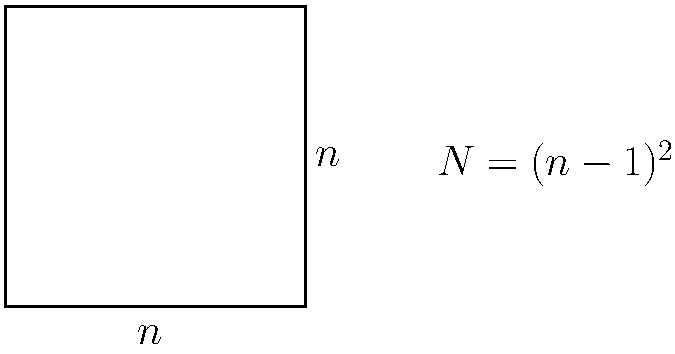
\includegraphics[width=6.5cm]{Domain2D_ntimesn}
\end{figure}

\begin{align*}
  \tau(n) &= \text{ total simulation time (in seconds)} \\
  \tau_1(n) &= \frac{\tau(n)}{n^2} \\
  r(n) &= \frac{\tau_1(n)}{\tau_1(\frac{n}{2})}
\end{align*}

\begin{table}[h]
  \begin{center}
    \begin{tabular}{|r!{\vrule width 3pt}l|l|l!{\vrule width 3pt}l|l|}
      \hline
      \multicolumn{1}{|r!{\vrule width 3pt}}{} & \multicolumn{3}{c!{\vrule width 3pt}}{PC (2000)} & \multicolumn{2}{c|}{gridur (2006)} \\
      \hline
      $n$ & $\tau(n)$ & $\tau_1(n)$ & $r(n)$ & $\tau(n)$ & $\tau_1(n)$ \\
      \hline
      $32$ & $1.80 \cdot 10^{-2}$ & $1.76 \cdot 10^{-5}$ & & &\\
      $64$ & $1.50 \cdot 10^{-1}$ & $3.66 \cdot 10^{-5}$ & $2.1$ & & \\
      $128$ & $1.20$ & $7.34 \cdot 10^{-5}$ & $2.0$ & $2.45 \cdot 10^{-2}$ & $1.50 \cdot 10^{-6}$ \\
      $256$ & $9.84$ & $1.50 \cdot 10^{-4}$ & $2.0$ & $0.167$ & $2.55 \cdot 10^{-6}$ \\
      $512$ & $103.9$ & $3.96 \cdot 10^{-4}$ & $2.6$ & $1.33$ & $5.08 \cdot 10^{-6}$ \\
      $1024$ & $873.2$ & $8.33 \cdot 10^{-4}$ & $2.1$ & $10.33$ & $9.85 \cdot 10^{-6}$ \\
      \hline
      & $\tau(n) \sim \mathcal{O}(n^3)$ & $\tau_1(n) \sim \mathcal{O}(n)$ & & & \\
      \hline
    \end{tabular}
  \end{center}
  \caption{Simulation results for the numerical approximation of the two-dimensional Poisson equation by finite differences. The solution of the system of discrete equations 
  is based on diagonalization techniques and matrix-matrix products. 
  A listing of the FORTRAN program used in these tests is given below. 
  It is interesting to note that 
  the elapsed time on a single processor on gridur is reduced by a factor of more than 
  80 compared to using the PC from 2000 when $n=1024$.}
\end{table}

\newpage
\begin{verbatim}
      program poisson
c
c     Program to solve the two-dimensional Poisson equation on 
c     a unit square using one-dimensional eigenvalue decompositions 
c     and matrix-vector products. 
c     In this example, the right hand side f=1.
c
c     einar m. ronquist
c     ntnu, october 2000
c
      parameter (n = 256)
      parameter (m = n-1)
c
      real*8 diag(m), q(m,m), qt(m,m), b(m,m), u(m,m), w(m,m), pi
      real*4 tarray(2), t1, t2, dt

      t1   = etime (tarray)

      h    = 1./n
      pi   = 4.*atan(1.)

      do i=1,m
         diag(i) = 2*(1-cos(i*pi/n))
      enddo

      do j=1,m
         do i=1,m
            q(i,j) = sin(i*j*pi/n) * sqrt((2./n))
         enddo
      enddo

      do j=1,m
         do i=1,m
            qt(i,j) = q(j,i)
         enddo
      enddo
            
      do j=1,m
         do i=1,m
            b(i,j) = h*h
         enddo
      enddo
      
      call mxm (b,m,q,m,w,m)
      call mxm (qt,m,w,m,b,m)
      
      do j=1,m
         do i=1,m
            u(i,j) = b(i,j)/(diag(i)+diag(j))
         enddo
      enddo

      call mxm (u,m,qt,m,w,m)
      call mxm (q,m,w,m,u,m)


      t2 = etime (tarray)
      dt = t2-t1
      write(6,*) ' ' 
      write(6,*) 'dt (total)= ',dt
      dt = dt/(n*n)
      write(6,*) 'dt (per dof)= ',dt

      stop
      end



      subroutine mxm (a,n1,b,n2,c,n3)
c
c     matrix-matrix product c = a*b
c
      real*8 a(n1,n2), b(n2,n3), c(n1,n3)
      do j=1,n3
         do i=1,n1
               c(i,j) = 0.0
               do k=1,n2
                  c(i,j) = c(i,j) + a(i,k)*b(k,j)
               enddo
         enddo
      enddo
      
      return
      end
\end{verbatim}


%%%%%%%%%%%%%%%%%%%%%%%%%%%%%%%%%%
\newpage 
\subsection{Fast diagonalization methods}

The most expensive operation in the diagonalization method introduced in the previous section is of the type,

\begin{align*}
  \underline{v}^* &= \underline{\mathbf{Q}} \underline{v} = \underline{\mathbf{Q}}^T \underline{v}, \\
  \intertext{where}
  Q_{ij} &= \sqrt{\frac{2}{n}} \sin \biggl( \frac{ij \pi}{n} \biggr) \qquad \qquad 1 \leq i,j \leq n-1.
\end{align*}

We will now consider ways to obtain $\underline{v}^*$ in $\mathcal{O}(n \log n)$ operations instead of $\mathcal{O}(n^2)$.


\subsubsection{Discrete Fourier Transform (DFT)}

Consider a periodic function $v(x)$ with period $2 \pi$. Consider sampling this function at the equidistant points $x_j, \quad j=0,1,\ldots,N,$ with $x_j=j h, \quad h=\frac{2 \pi}{N}$. Let $v_j = v(x_j) = v(j h), \quad j=0,1,\ldots,N$.

\begin{figure}[h]
  \centering
  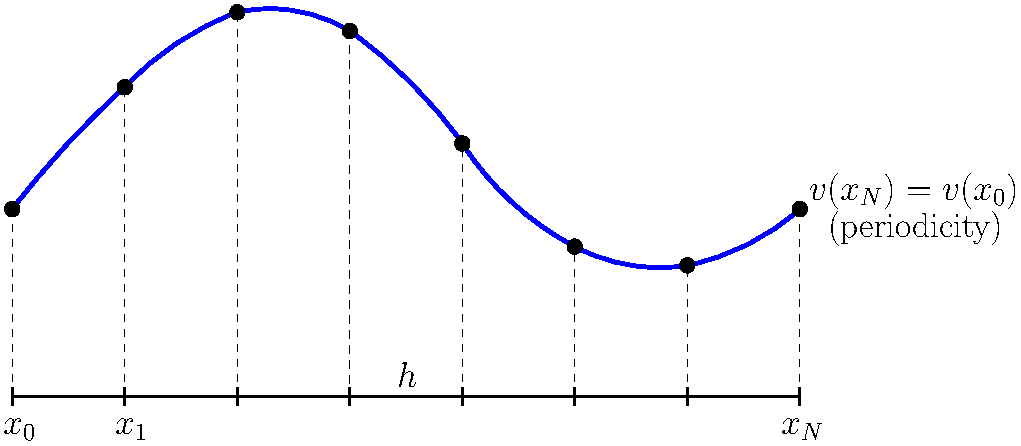
\includegraphics[width=10cm]{PeriodicFunction}
\end{figure}


Consider the vectors $\underline{\varphi}_k$, where

\begin{equation*}
  (\underline{\varphi}_k)_j = e^{i k x_j}, \qquad j,k=0,1,\ldots,N-1.
\end{equation*}

Note that the vector elements in $\underline{\varphi}_k$ represent the values of the function $\varphi_k(x) = e^{ikx}$ sampled at the discrete points $x_j, \quad j=0,1,\ldots,N-1$. Note also that the function $\varphi_k(x) = e^{ikx}$ is an eigenfunction of the Laplace operator with periodic boundary conditions.

The vectors $\{ \underline{\varphi}_k \}_{k=0}^{N-1}$ form a basis for the $N$-dimensional  vector space $\mathbb{C}^N$. In particular, we have that 

\begin{equation*}
  \underline{\varphi}_k^H \underline{\varphi}_l = 
  \begin{cases}
    N, & k=l, \\
    0, & k \not= l,
  \end{cases}
  \qquad \qquad k,l=0,1,\ldots,N-1.
\end{equation*}
    
The vector 

\begin{equation*}
  \underline{v} = 
  \begin{bmatrix}
    v_0 \\
    \vdots \\
    v_{N-1}
  \end{bmatrix}
  \in \mathbb{R}^N
\end{equation*}

can be expressed in this basis as

\begin{align*}
  \underline{v} &= \sum_{k=0}^{N-1} \hat{v}_k \underline{\varphi}_k \\
  \intertext{or}
  v_j &= \sum_{k=0}^{N-1} \hat{v}_k (\underline{\varphi}_k)_j = \sum_{k=0}^{N-1} \hat{v}_k e^{ik x_j},
\end{align*}

where $\hat{v}_k$, are the discrete Fourier coefficients given by

\begin{equation*}
  \hat{v}_k = \frac{1}{N} \sum_{j=0}^{N-1} v_j e^{-ik x_j}, \qquad \qquad 
  \begin{matrix}
    x_j = j h \\
    h = \frac{2\pi}{N}
  \end{matrix}
  \qquad k=0,1,\ldots,N-1
\end{equation*}
  
\underline{\textbf{Summary (DFT)}}:

\begin{alignat*}{2}
  v_j &= \sum_{k=0}^{N-1} \hat{v}_k e^{ijkh}, & \qquad \qquad j&=0,1,\ldots,N-1, \\
  \intertext{where}
  \hat{v}_k &= \frac{1}{N} \sum_{j=0}^{N-1} v_j e^{-ijkh}, & \qquad \qquad k&=0,1,\ldots,N-1, \\
  \intertext{and}
  h &= \frac{2 \pi}{N}.
\end{alignat*}


\subsubsection{Discrete Sine Transform (DST)}

The Discrete Sine Transform is applicable to a function $v(x)$ which is \underline{periodic} with period $2 \pi$ and \underline{odd}. Discretize the function on an equidistant grid on $[0,\pi]$ with $h=\frac{\pi}{n}$. Set

\begin{equation*}
  v_j = v(x_j) = v(jh) = v \biggl(\frac{j \pi}{n} \biggr), \qquad \qquad j=0,1,\ldots,n.
\end{equation*}

Since $v$ is odd,

\begin{equation*}
  v(x_0) = v(x_n) = 0.
\end{equation*}

The discretized function is therefore represented by the $(n-1)$ real values $v_1,\ldots,v_{n-1}$, i.e., by the vector

\begin{equation*}
  \underline{v} = 
  \begin{bmatrix}
    v_1 \\
    \vdots \\
    v_{n-1}
  \end{bmatrix}
  \in \mathbb{R}^{n-1}.
\end{equation*}

An orthogonal basis for $\mathbb{R}^{n-1}$ is given by the vectors $\underline{\psi}_k, \quad k=1,\ldots,n-1$, where

\begin{align*}
  (\underline{\psi}_k)_j &= \sin \biggl( \frac{k j \pi}{n} \biggr), \qquad j=1,\ldots,n-1, \\
  \intertext{and with}
  \underline{\psi}_k^T \underline{\psi}_l &=
  \begin{cases}
    \frac{n}{2}, & k=l, \\
    0, & k \not= 0.
  \end{cases}
\end{align*}

In terms of this basis, we can write $\underline{v}$ as

\begin{alignat*}{2}
  v_j &= \sum_{k=1}^{n-1} \widetilde{v}_k \sin \biggl( \frac{k j \pi}{n} \biggr), &\qquad j&=1,\ldots,n-1, \\
  \intertext{where}
  \widetilde{v}_k &= \frac{2}{n} \sum_{j=1}^{n-1} v_j \sin \biggl( \frac{j k \pi}{n} \biggr), &\qquad  k&=1,\ldots,n-1.
\end{alignat*}

We can also write this as

\begin{align*}
  \underline{\widetilde{v}} &= \underline{\mathbf{S}} (\underline{v}) \qquad (\text{DST}). \\
  \intertext{and}
  \underline{v} &= \underline{\mathbf{S}}^{-1} (\underline{\widetilde{v}}) \qquad (\text{inverse DST}).
\end{align*}

Note that $\underline{\mathbf{S}}(\cdot)$ and $\underline{\mathbf{S}}^{-1}(\cdot)$ are related as 

\begin{equation*}
  \boxed{
    \underline{\mathbf{S}} = \frac{2}{n} \underline{\mathbf{S}}^{-1}
  }
\end{equation*}

Also note that

\begin{align*}
  \underline{\mathbf{Q}} &= \sqrt{\frac{2}{n}} \underline{\mathbf{S}}^{-1}, \\ 
  \intertext{and}
  \underline{\mathbf{Q}} = \sqrt{\frac{2}{n}} \underline{\mathbf{S}}.
\end{align*}

Now, consider the matrix $\underline{\mathbf{F}}^{(N)}$ where

\begin{equation*}
  \begin{split}
    F_{k,j}^{(N)} &= e^{-ijkh} \\
    &= \cos \biggl( \frac{j k 2 \pi}{N} \biggr) - i \sin \biggl( \frac{j k 2 \pi}{N} \biggr), \qquad 0 \leq j,k \leq N-1.
  \end{split}
\end{equation*}

Note that

\begin{equation*}
  F_{k,j}^{(2 n)} = \cos \biggl( \frac{j k \pi}{n} \biggr) - i \sin \biggl( \frac{j k \pi}{n} \biggr), \qquad 0 \leq j,k \leq 2n-1.
\end{equation*}

Now, consider

\begin{align*}
  \underline{v} &= 
  \begin{bmatrix}
    v_1 \\
    \vdots \\
    v_{n-1}
  \end{bmatrix}
  \in \mathbb{R}^{n-1}. \\
  \intertext{Construct the extended vector as an ``odd'' extension}
  w &=
  \begin{bmatrix}
    0 \\ 
    v_1 \\
    \vdots \\
    v_{n-1} \\
    0 \\
    -v_{n-1} \\
    \vdots \\
    -v_1
  \end{bmatrix}
  \in \mathbb{R}^{2n}.
\end{align*}

First, note that

\begin{equation*}
  (\underline{\mathbf{F}}^{(2n)} \underline{w})_k = \sum_{j=0}^{2n-1} e^{\frac{-ijk \pi}{n}} w_j = 2n \hat{w}_k,
\end{equation*}
where $\hat{w}, \quad k=0,1,\ldots,2n-1$, are the discrete Fourier coefficients. Second,

\begin{align*}
  (\underline{\mathbf{F}}^{(2n)} \underline{w})_k &= \sum_{j=0}^{2n-1} \biggl[ \cos \biggl( \frac{j k \pi}{n} \biggr) - i \sin \biggl( \frac{jk \pi}{n} \biggr) \biggr] w_j \\
  &= \sum_{j=0}^{2n-1} \underset{\text{odd}}{\underset{\uparrow}{w_j}} \underset{\text{even}}{\underset{\uparrow}{\cos}} \biggl( \frac{jk \pi}{n} \biggr) - i \sum_{j=0}^{2n-1} \underset{\text{odd}}{\underset{\uparrow}{w_j}} \underset{\text{odd}}{\underset{\uparrow}{\sin}} \biggl( \frac{j k \pi}{n} \biggr) \\
  &= -2i \sum_{j=0}^{n-1} w_j \sin \biggl( \frac{j k \pi}{n} \biggr) \\
  &= -2i \sum_{j=1}^{n-1} w_j \sin \biggl( \frac{j k \pi}{n} \biggr) \qquad (\text{since } w_0=0).
\end{align*}

Hence

\begin{equation*}
  \frac{i}{2} ( \underline{\mathbf{F}}^{(2n)} \underline{w})_k = \sum_{j=1}^{n-1} w_j \sin \biggl( \frac{j k \pi}{n} \biggl) = \frac{n}{2} \widetilde{w}_k.
\end{equation*}

Since 

\begin{equation*}
  w_j=v_j, \qquad j=1,\ldots,n-1,
\end{equation*}

it follows that

\begin{equation*}
  \widetilde{w}_k = \widetilde{v}_k, \qquad k=1,\ldots,n-1.
\end{equation*}

In summary, for $k=1,\ldots,n-1$,

\begin{align*}
  \widetilde{v}_k = \widetilde{w}_k &= \frac{2}{n} \frac{i}{2} (\underline{\mathbf{F}}^{(2n)} \underline{w})_k \\
  &= \frac{i}{n} (\underline{\mathbf{F}}^{(2n)} \underline{w})_k \\
  &= \frac{i}{n} 2n \hat{w}_k \\
  &= 2i \hat{w}_k.
\end{align*}

By computing the discrete Fourier coefficients $\hat{w}_k$, we can find the discrete sine coefficients $\widetilde{v}_k, \quad k=1,\ldots,n-1,$ where

\begin{equation*}
  \underline{\widetilde{v}}=\underline{\mathbf{S}}(\underline{v}) = \sqrt{\frac{2}{n}} \underline{\mathbf{Q}} \underline{v}.
\end{equation*}

The operator $(\underline{\mathbf{F}}^{(2n)} \underline{w})$ can be computed efficiently by a FFT in $\mathcal{O}(2n \log 2n) \sim \mathcal{O} (n \log n)$ operations.

This leads to the \underline{modified algorithm} (Poisson solver):

\renewcommand{\theenumi}{\arabic{enumi}}
\renewcommand{\labelenumi}{\textbf{\theenumi)}}
\begin{enumerate}
  \item
    \begin{align*}
      \underline{\widetilde{\mathbf{G}}} &= \underline{\mathbf{Q}}^T \underline{\mathbf{G}} \underline{\mathbf{Q}} \\
      \Rightarrow \quad \underline{\widetilde{\mathbf{G}}}^T &= \underline{\mathbf{Q}}^T \underline{\mathbf{G}}^T \underline{\mathbf{Q}} \\
      &= \underline{\mathbf{Q}} \underline{\mathbf{G}}^T \underline{\mathbf{Q}}^T \qquad (\underline{\mathbf{Q}}=\underline{\mathbf{Q}}^T) \\
      &= \underline{\mathbf{Q}} (\underline{\mathbf{Q}} \underline{\mathbf{G}})^T \\
      &= \sqrt{\frac{2}{n}} \underline{\mathbf{S}}^{-1} \biggl( \biggl( \sqrt{\frac{n}{2}} \underline{\mathbf{S}}( \underline{\mathbf{G}}) \biggr)^T \biggr) \\
      &= \underline{\mathbf{S}}^{-1} ((\underline{\mathbf{S}} (\underline{\mathbf{G}}))^T) \qquad \qquad \qquad \qquad \qquad \qquad \mathcal{O}(n^2 \log n)
    \end{align*}

  \item
    \begin{equation*}
      \widetilde{U}_{ji} = \frac{\widetilde{G}_{ji}}{\lambda_j+\lambda_i} \qquad \qquad \qquad \qquad \qquad \qquad \qquad \quad \mathcal{O}(n^2)
    \end{equation*}

  \item
    \begin{align*}
      \underline{\mathbf{U}} &= \underline{\mathbf{Q}} \underline{\mathbf{\widetilde{U}}} \underline{\mathbf{Q}}^T \\
      &= \underline{\mathbf{Q}} ( \underline{\mathbf{Q}} \underline{\mathbf{\widetilde{U}}}^T)^T \\
      &= \underline{\mathbf{S}}^{-1}((\underline{\mathbf{S}}(\underline{\mathbf{\widetilde{U}}}^T))^T) \qquad \qquad \qquad \qquad \qquad \qquad \qquad \mathcal{O}(n^2 \log n)
    \end{align*}
\end{enumerate}

Again,

\begin{equation*}
  \underline{\mathbf{S}} = \frac{2}{n} \underline{\mathbf{S}}^{-1}
\end{equation*}

and $\underline{\widetilde{v}} = \underline{\mathbf{S}} \, \underline{v}$ is obtained as follows

\renewcommand{\theenumi}{\roman{enumi}}
\renewcommand{\labelenumi}{\textbf{\theenumi)}}

\begin{enumerate}
  \item
    \begin{equation*}
      \underline{v} \in \mathbb{R}^{n-1} \quad \rightarrow \quad \underline{w} \in \mathbb{R}^{2n} 
    \end{equation*}

  \item
    \begin{equation*}
      \text{Compute } \underline{\hat{w}} \text{ via FFT } (\mathcal{O}(n \log n)).
    \end{equation*}
  \item
    \begin{equation*}
      \widetilde{v}_k = 2i \hat{w}_k, \qquad k=1,\ldots,n-1.
    \end{equation*}

\end{enumerate}

\newpage
\subsubsection{Numerical results}

\renewcommand{\theenumi}{$\bullet$}
\renewcommand{\labelenumi}{\theenumi}
\begin{enumerate}
  \item
    Diagonalization

  \item
    DST (FFT)

  \item
    PC, Pentium III, 512 MB RAM

 \end{enumerate}
   
\begin{figure}[h]
  \centering
  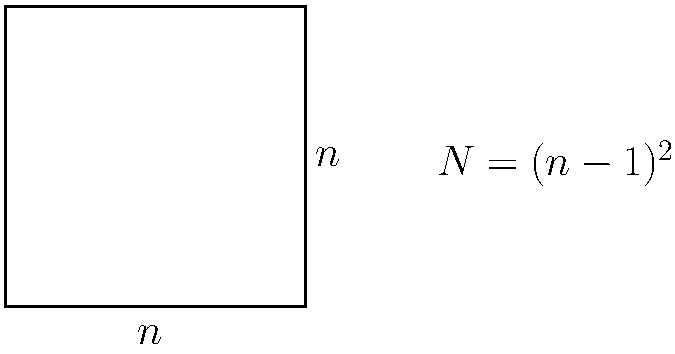
\includegraphics[width=8cm]{Domain2D_ntimesn}
\end{figure}

\begin{align*}
  \tau^n &= \text{ total simulation time (in seconds)} \\
  \tau_1^n &= \frac{\tau}{n^2} 
\end{align*}

\begin{table}[h]
  \begin{center}
    \begin{tabular}{|r|l|l|l|}
      \hline
      $n$ & $\tau^n$ & $\tau_1^n$ & $\tau_1^n (m \times m)$ \\
      \hline
      $32$ & $2.36 \cdot 10^{-2}$ & $2.31 \cdot 10^{-5}$ & $1.76 \cdot 10^{-5}$ \\
      $64$ & $1.11 \cdot 10^{-1}$ & $2.71 \cdot 10^{-5}$ & $3.66 \cdot 10^{-5}$ \\
      $128$ & $5.19 \cdot 10^{-1}$ & $3.17 \cdot 10^{-5}$ & $7.34 \cdot 10^{-5}$ \\
      $256$ & $2.35$ & $3.58 \cdot 10^{-5}$ & $1.50 \cdot 10^{-4}$ \\
      $512$ & $10.5$ & $3.99 \cdot 10^{-5}$ & $3.96 \cdot 10^{-4}$ \\
      $1024$ & $46.2$ & $4.41 \cdot 10^{-5}$ & $8.33 \cdot 10^{-4}$ \\
      \hline
      & $\tau^n \sim \mathcal{O}(n^2 \log n)$ & $\tau_1^n \sim \mathcal{O}(\log n)$ & $\tau_1^n \sim \mathcal{O}(n) $ \\
      \hline
    \end{tabular}
  \end{center}
  \caption{Simulation results for the numerical approximation of the two-dimensional Poisson equation by the use of fast diagonalization techniques.}
\end{table}

\newpage
\begin{verbatim}
      program poisson
c==================================================================
c
c     FORTRAN-program to solve the two-dimensional Poisson equation 
c     on a unit square using finite differences (five-point stencil), 
c     one-dimensional eigenvalue decompositions and fast sine transforms. 
c     In this example, the right hand side f=1. 
c
c     note: n needs to be a power of 2
c
c     einar m. ronquist
c     ntnu, october 2000
c
c===================================================================
      parameter (n  = 256)
      parameter (m  = n-1)
      parameter (nn = 4*n)
c
      real*8    diag(m), b(m,m), bt(m,m) 
      real*8    pi
      real*8    z(0:nn-1)
      real*4    tarray(2), t1, t2, dt

      h    = 1./n
      pi   = 4.*datan(1.)

      do i=1,m
         diag(i) = 2*(1-dcos(i*pi/n))
      enddo
            
      do j=1,m
         do i=1,m
            b(i,j) = h*h
         enddo
      enddo
      
      \end{verbatim}
      \newpage
      \begin{verbatim}      
      do j=1,m
         call fst (b(1,j), n, z, nn)
      enddo 
      call transp (bt, b, m)
      do i=1,m
         call fstinv (bt(1,i), n, z, nn)
      enddo 


      do j=1,m
         do i=1,m
            bt(i,j) = bt(i,j)/(diag(i)+diag(j))
         enddo
      enddo


      do i=1,m
         call fst (bt(1,i), n, z, nn)
      enddo 
      call transp (b, bt, m)
      do j=1,m
         call fstinv (b(1,j), n, z, nn)
      enddo 



      umax = 0.0
      do j=1,m
         do i=1,m
            if (b(i,j) .gt. umax) umax = b(i,j)
         enddo
      enddo

      write(6,*) ' ' 
      write(6,*) umax

      stop
      end

\end{verbatim}
\newpage
\begin{verbatim}

      subroutine transp (at, a, m)
c====================================================
c     set at equal to the transpose of a 
c====================================================
      real*8 a(m,m), at(m,m)

      do j=1,m
         do i=1,m
            at(j,i) = a(i,j)
         enddo
      enddo
      return
      end



\end{verbatim}

\end{document}
